\documentclass[10pt]{article}
\usepackage[margin = 1in]{geometry}
\usepackage{xcolor}
\usepackage{fancyhdr}
% \usepackage{tgschola} % or any other font package you like
\usepackage{lastpage}
\usepackage{parskip} % Remove paragraph indentation
\usepackage{amsmath} % for align
\usepackage{amsthm} % for proof pkg
\usepackage{amssymb}
%\usepackage{tikz}
\usepackage{graphicx}
\usepackage{proof}
\usepackage{enumitem}
% \usepackage[shortlabels]{enumerate}
\usepackage{algorithm}
\usepackage{algorithmicx}
\usepackage{algpseudocode}
\usepackage{hyperref}
\usepackage{subcaption}
 \usepackage{setspace}
 \usepackage{url}
 \usepackage[square,sort,comma,numbers]{natbib}
 \usepackage{apalike}
 \usepackage{helvet}
 \usepackage{titling}
 
 \usepackage{paralist}
% \usepackage[compact]{titlesec}
 %\titlespacing{\section}{0pt}{8pt minus 2pt}{0pt minus 2pt}
 %\titlespacing{\subsection}{0pt}{8pt minus 2pt}{0pt minus 2pt}
 %\titlespacing{\subsubsection}{0pt}{8pt minus 2pt}{0pt minus 2pt}
 
 
 %\linespread{0.95}
 %\addtolength{\belowcaptionskip}{-2mm}
 %\addtolength{\itemsep}{-3mm}


% Natbib setup for author-year style
\usepackage{natbib}
%\bibpunct[, ]{(}{)}{,}{a}{}{,}%
\bibpunct{[}{]}{,}{a}{}{;}
\def\bibfont{\small}%
\def\bibsep{\smallskipamount}%
\def\bibhang{24pt}%
\def\newblock{\ }%
\def\BIBand{and}%



\newtheorem{theorem}{Theorem}
\newtheorem{corollary}{Corollary}
\newtheorem{lemma}{Lemma}
\newtheorem{proposition}{Proposition}
\newtheorem{remark}{Remark}
\newtheorem{example}{Example}

\renewcommand{\algorithmicrequire}{\textbf{Input:}}  % Use Input in the format of Algorithm
\renewcommand{\algorithmicensure}{\textbf{Output:}} % Use Output in the format of Algorithm  
\newtheorem{claim}{Claim}


%\newcommand{\yourtitle}{Contagion in Reinsurance Networks}







%\onehalfspacing


\title{Proposal: A Framework for Designing Better Stablecoins
}

\author{Ariah Klages-Mundt}

\date{\today}



\begin{document}


\maketitle


\abstract{
I propose to develop a framework for understanding stablecoin markets. Through this framework, we will be able to compare the performances of different stablecoin designs and parameter choices and better understand the settings under which stablecoins can work and fail. Toward this, I also contribute a new decentralized stablecoin design, which we will be able to evaluate and tune using the framework I will develop. This grant will help me to perform this research, which is a step toward building new stablecoins that achieve better long-term stability by making informed design choices.
}


%%%%%%%%%%%%%%%%%%%%%%%%%%%%%%%%%%%%%%
\section{Introduction}

A stablecoin is a cryptocurrency with an economic structure built on top of blockchain that aims to stabilize the trading price of the coin. A true stablecoin would offer the benefits of cryptocurrencies (cryptographic security, privacy, incentive alignment, digital usability, and accessibility to the unbanked) without the unusable volatility. This could form the basis for a robust decentralized financial system and facilitate economic adoption of cryptocurrencies. In the short term, stablecoins fulfill a stop-gap measure to make cryptocurrencies usable. In a mature cryptoeconomy, a stablecoin may still have a place as we may want a currency that can adapt to agreed upon economic measures to enable some benefits of monetary policy (e.g., a coin supply that can adapt to changing circumstances).


\paragraph{Cryptocurrency volatility}
Cryptocurrencies face difficult technological, usability, and regulatory challenges to be successful in longterm. There are many competing cryptocurrency systems that attempt different approaches to solving these problems. Even if the crypto space is successful in the long run, there is huge uncertainty about the long term value of individual systems--ranging from very high to zero. It's hard to predict which systems will ultimately be adopted. Holding a cryptocurrency in the short term is a very speculative bet on a specific version of new technology. Further, the decentralized control and privacy features of cryptocurrencies can be at odds with desires of governments, who could attempt interventions in the space.

This price volatility feeds back into fundamental usability problems. It makes cryptocurrencies unusable as good stores of value. This makes it harder for cryptocurrencies to be adopted as potential users see that it doesn't perform its intended purpose well. Indeed, today we see that most cryptocurrency transactions represent speculative investment as opposed to typical economic activity.

The success of a cryptocurrency is based on network effects: the system becomes much more valuable in a nonlinear way as new participants join. In concrete terms, the more people who use the system, the more likely it can be used to fulfill a given real world transaction. Further, the more people who treat a floating digital asset as a good store of value, the better a store of value it will be. Indeed, it took society a while (and multiple times) to settle on gold as a good store of value. Most recently, this can be seen in the high volatility of gold prices after the Federal Reserve abandoned the gold standard. This volatility eventually settled down as society decided that gold still had value. To become digital gold, a cryptocurrency relies on a mass of people treating it that way. To become a global currency, a cryptocurrency additionally relies on a mass of merchants and businesses adopting the system for transactions. The value of these systems is, to some degree, self-fulfilling.


\paragraph{Existing stablecoin designs are fragile}
Current stablecoins bootstrap existing ideas from traditional finance into a blockchain setting, introducing new and unaddressed failure points (more details about this in Section~\ref{sec:existing_designs}):
\begin{compactenum}
\item Centralized designs rely on trusted institutions to hold reserve assets off-chain and/or report off-chain market data to the blockchain (called an "oracle", which might report e.g. USD prices). These institutions are susceptible to failure, hacking, and fraud. Blockchain was supposed to solve this counterparty risk.
\item Decentralized designs create complicated and poorly designed systems of financial contracts backed by volatile cryptocurrencies. These systems are prone to extreme liquidity crises (similar to traditional banking crises), in which speculative agents may no longer be willing to take opposing sides of stabilizing trades. This causes unrecoverable failure in these systems.
\end{compactenum}

An example of the centralized risk is the recent volatility in Tether, falling as low as \href{https://www.ccn.com/bitcoin-price-explodes-to-7500-as-tether-loses-usd-peg/}{\$0.85 in October 2018} and consistently facing a \href{https://www.lykke.com/trading-indicators}{$\sim3\%$ premium on BTC/Tether markets vs. BTC/fiat markets}. NuBits, which current trades at cents on the dollar (Figure~\ref{fig:nubits_chart}), is a recent example of extreme failure of decentralized designs. BitUSD and Steem Dollars, other decentralized designs, have also recently broken their USD peg (Figure~\ref{fig:bitusd_chart}). I discuss these events in the Medium article \href{https://medium.com/@aklamun/the-state-of-stablecoins-update-2018-56fb82efe6de}{``The State of Stablecoins--Dec 2018''}.

\begin{figure}
	\centering
	\begin{subfigure}[b]{0.48\textwidth}
		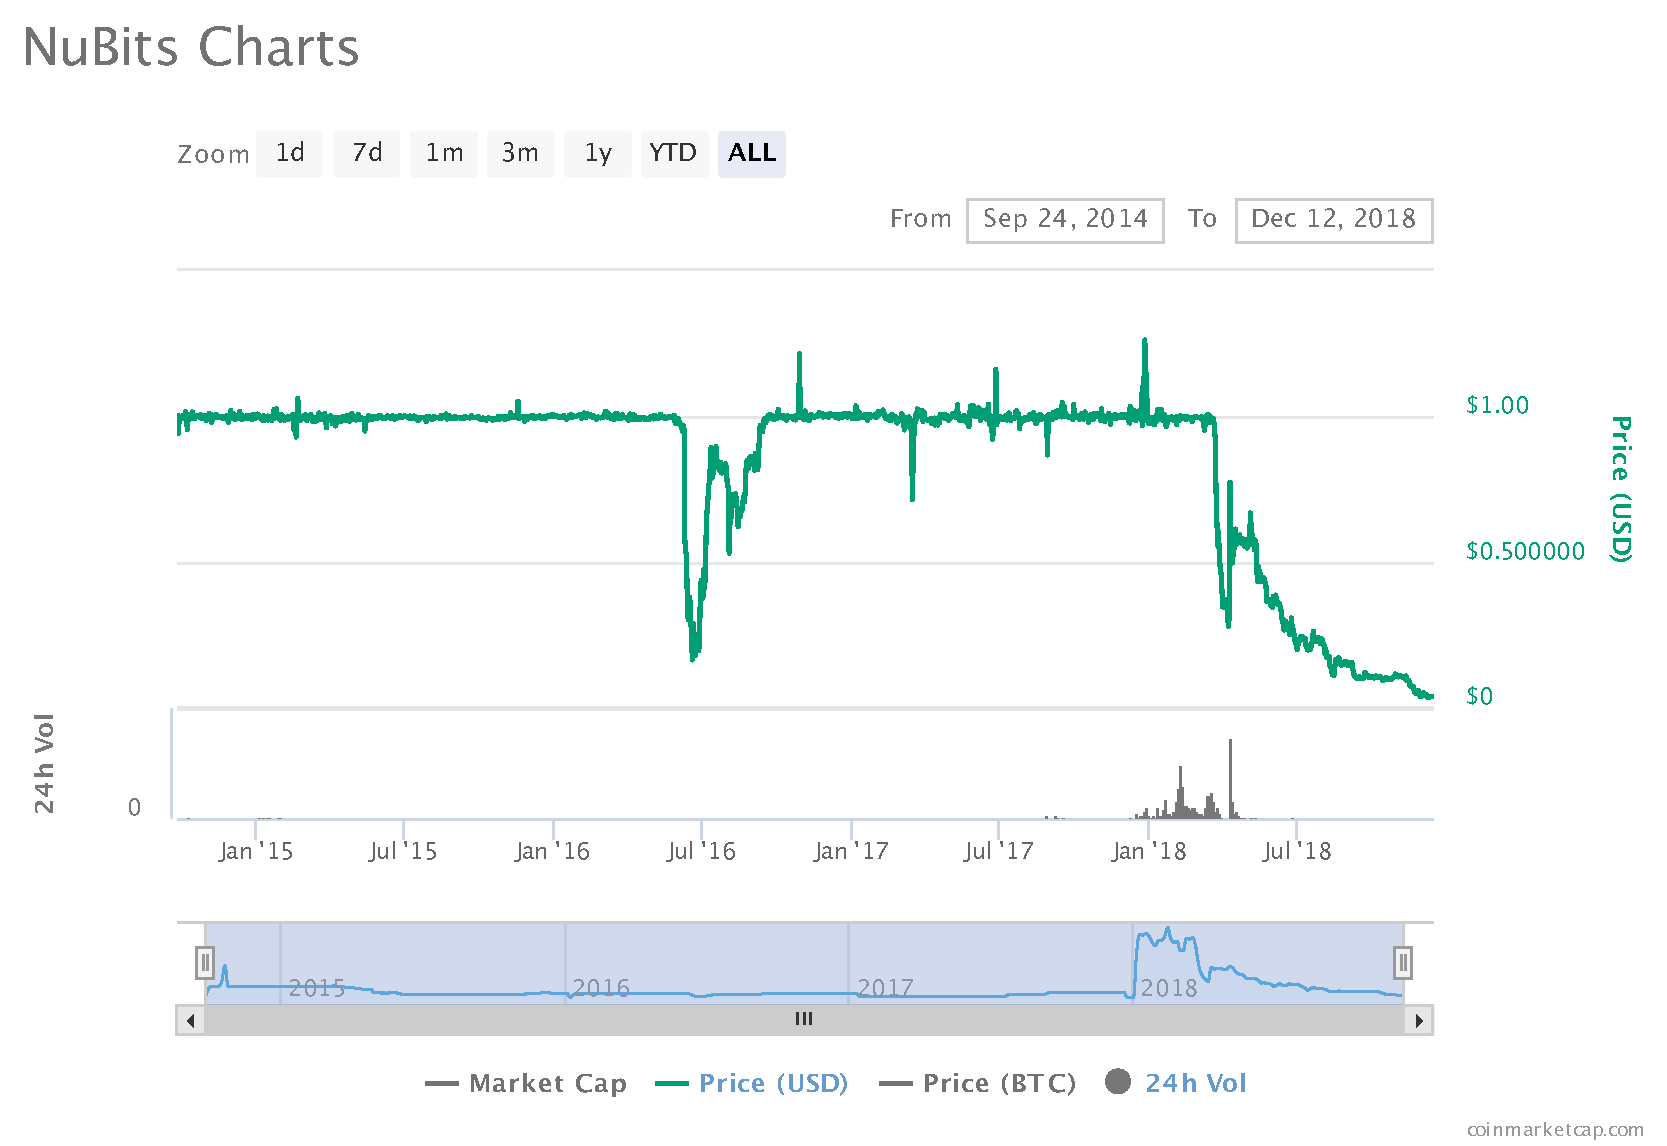
\includegraphics[width=\textwidth]{nubits_chart}
		\caption{NuBits stablecoin is trading at \$0.04 on the dollar.}\label{fig:nubits_chart}
	\end{subfigure}
	%
	\begin{subfigure}[b]{0.48\textwidth}
		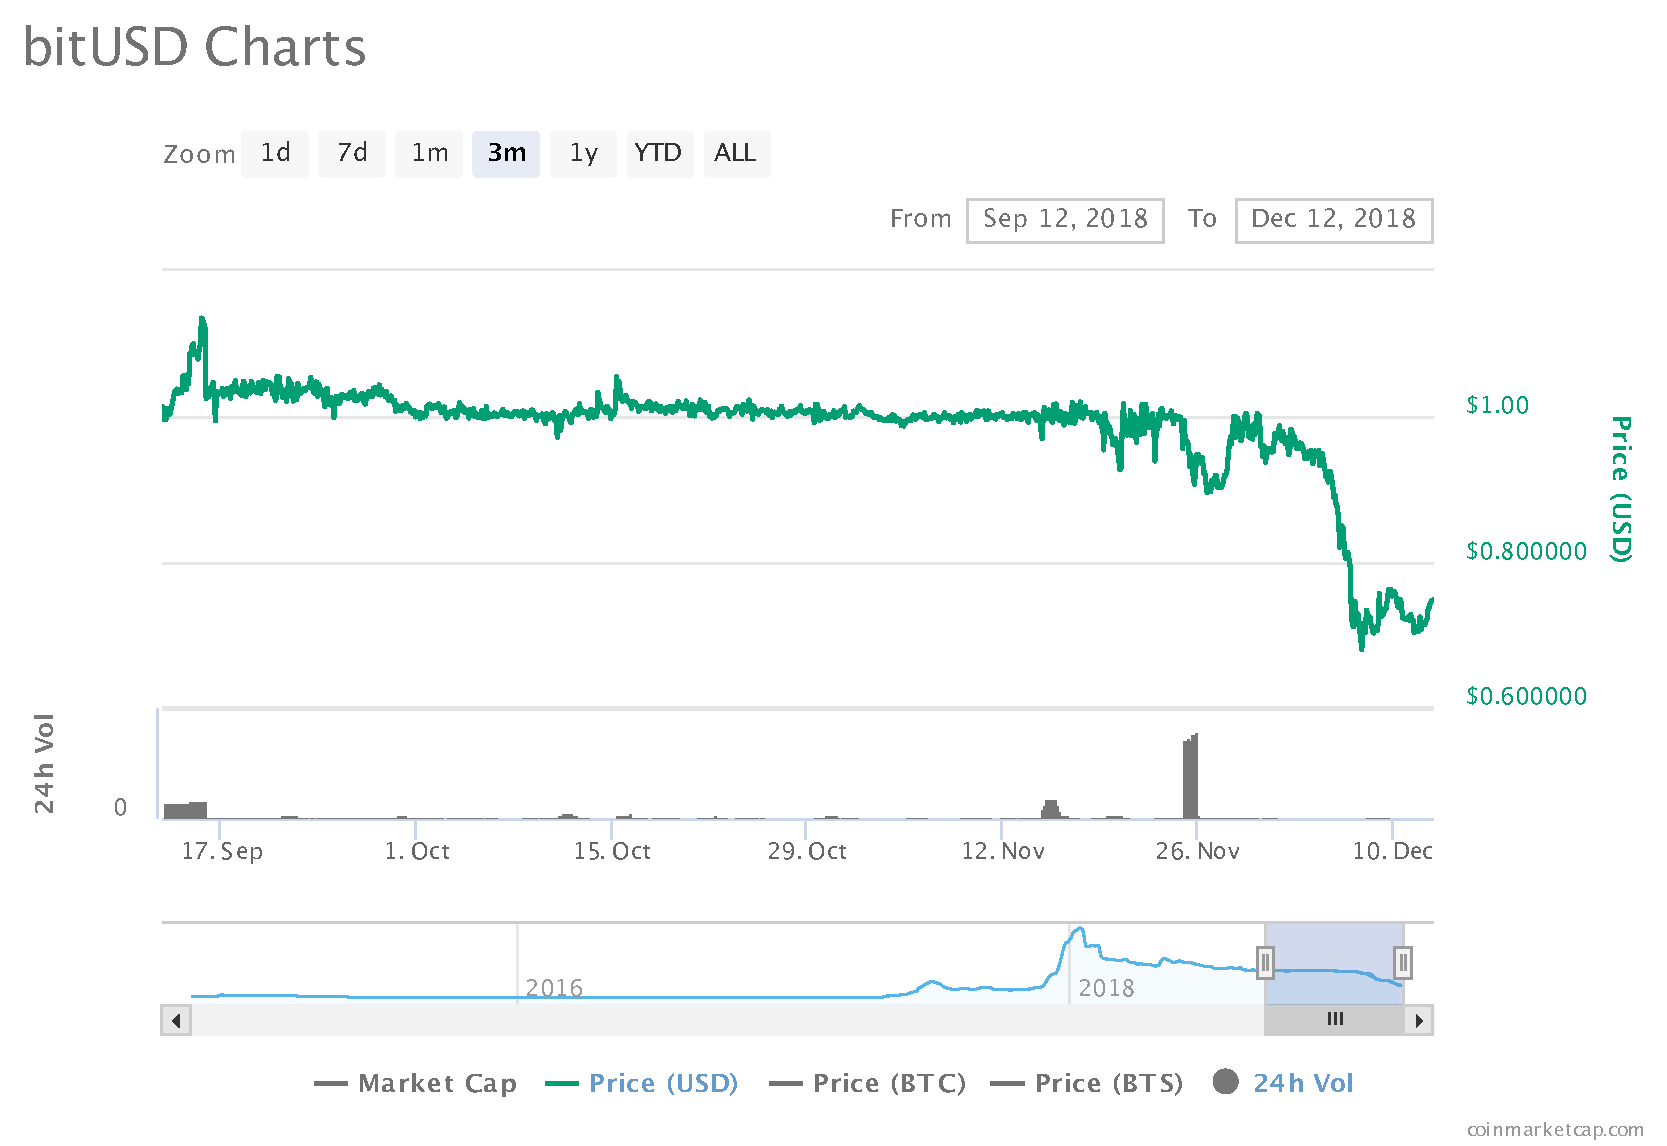
\includegraphics[width=\textwidth]{bitusd_chart}
		\caption{BitUSD has broken its USD peg.}\label{fig:bitusd_chart}
	\end{subfigure}
	\caption{Recent decentralized stablecoin failures.}
\end{figure}


\paragraph{The current stablecoin space}
Despite the long term stability issues and past failures, there is huge interest to develop new stablecoins using the same basic designs. For instance, Basis recently raised \$133M to build a design substantially similar to NuBits.\footnote{As of Dec. 2018, \href{https://cointelegraph.com/news/major-stablecoin-basis-to-close-return-funds-to-investors-sources}{Basis will actually be closing down and returning money to investors}. This is attributed to regulatory concerns. Whether it is also tied to the failure of the similar stablecoin NuBits is unclear.} The design focus has been on developing features that remain stable in median cases with little innovation toward things that continue to work during extreme crises. This is like working in an `assumed stable domain'--the same sort of thinking that led to the 2008 financial crisis. Ultimately, the success of stablecoins will depend on their ability to survive extreme events (the tails of the probability distribution instead of the center).

I believe that new thinking is needed in the stablecoin space to focus on long-term stability. In general, it is impossible to build a stablecoin system without significant risks. But we can focus on systems in which extreme events don't necessarily lead to system failure. In this regard, we want a system that has a fighting chance at surviving and recovering from extreme events and, ideally, grows stronger as a result--this is what Nassim Taleb calls an `anti-fragile' system.

The main impediment to moving forward with this thinking is that we don't really understand stablecoin markets very well. I'm not aware of any other work that aims to rigorously understand stablecoin markets (or more generally the sort of risk transfer markets that stablecoins represent). We only have informal ideas of how stablecoin designs work and fail. With this project, I plan to jumpstart foundational work in this area.


\paragraph{This project}
I propose to develop a framework for understanding stablecoin markets. Through this framework, we will be able to compare the performances of different stablecoin designs and parameter choices and better understand the settings under which stablecoins can work and fail. This research is a step toward developing the next generation of stablecoins that achieve better long-term stability by making informed design choices. Toward this, I contribute a new decentralized stablecoin design in Section~\ref{sec:new_design} and describe my research proposal in Section~\ref{sec:proposed_research}.

The contents of this proposal have been reviewed by several crypto founders and Ethereum experts, fellow PhD students, and several professors.



\paragraph{About me}
I am an applied math PhD student at Cornell University. My work is at the intersection of economics and computer science. I aim to better understand complex economic systems with the goal to design systems that survive extreme events. This has led to my interest in the design of cryptoeconomic systems and this project. My past work has focused on understanding cascades in networks of complex financial contracts, for which I have a paper under revision for \emph{Management Science}. Before starting my PhD, I worked in finance software developing fixed income risk models and economic classification tools. Prior to that, I studied math at Amherst College, focusing on number theory.

I have several academic collaborators. My PhD advisor Andreea Minca (operations research @ Cornell) will be directly involved with this research. Other primary collaborators, who may be involved with parts of the project, include Sven Seuken and Steffen Schuldenzucker (market design @ University of Zurich) and Yuchong Zhang (applied probability @ University of Toronto).











%%%%%%%%%%%%%%%%%%%%%%%%%%%%%%%%%%%%%%%%%%%%
\section{Existing Stablecoin Designs}\label{sec:existing_designs}


There are three main ideas behind price stability in existing designs:
\begin{compactitem}
	\item \textbf{Collateral} that guarantees the value of the stablecoin
	
	\item \textbf{Dynamic coin supply} that changes the number of coins in circulation as demand changes
	
	\item \textbf{Derivatives}, such as Collateralized Debt Obligations (CDO), that put seniority levels on a collateral pool, leading to a range of tokens from most stable to most volatile
\end{compactitem}
Existing stablecoins use combinations of these ideas, which I categorize in the following types.

\subsection{Centralized} 
In a centralized stablecoin, some central organization (usually a company) is trusted to hold a collateral reserve of real assets off-chain, such as fiat currency or gold. They then issue digital tokens that are tied to the reserve value in one of the following ways:
\begin{compactitem}
	\item Either the digital tokens are directly redeemable off-chain for the underlying real collateral.
	\item Or the centralized entity promises to control the money supply by either using reserve funds to buy coins when prices are below the collateral level or selling new coins and adding collateral to the reserve when prices are above the collateral level.
\end{compactitem}
Given $\geq 100\%$ collateralization, this is always possible. 

\paragraph{Counterparty risks} Holders of such a coin face counterparty risk in the following senses:
\begin{compactenum}
	\item The value of the coin can go to zero if the centralized entity is unable to fulfill its obligations, such as a result of fraud, mismanagement, theft, government seizure etc.
	\item The centralized entity can force arbitrary rules on coin holders, in aggregate or individually. In the extreme, this can potentially render an individual's coins useless.
\end{compactenum}
Financial institutions fail often enough for the first to be a serious concern. The second is a concern, for instance, if an individual is unjustifiably (i.e., without due process) placed on a blacklist. This realistically happens on centralized platforms like Airbnb and Uber and to the unbanked population. This is the result of an incentive mismatch: companies have little incentive to worry about individual cases or poor populations unless it is their explicit mission. By design, cryptocurrencies are supposed to solve both of these problems, so it's unfortunate to port them back into the system.

Examples include \href{https://tether.to/}{Tether}, \href{https://www.trusttoken.com/trueusd/}{TrueUSD}, \href{https://www.circle.com/en-gb/usdc}{USD Coin}, \href{https://gemini.com/dollar/}{Gemini Dollar}, and \href{https://www.paxos.com/standard/}{Paxos Standard}.

\paragraph{Government blockchain risks} In the future, governments may back centralized stablecoins similar to current fiat currencies. While this would improve many aspects of counterparty risk, it would also introduce very important problems. Governments would arguably construct these systems such that the government has complete control by design. This would include the ability to place arbitrary account restrictions, such as freezing of value, and would guarantee zero financial privacy for citizens. As a society, we would ideally have reasonable privacy and want `blacklist' sort of decisions to go through a communal process, such as the current judicial system. A government `cryptocurrency' that isn't carefully constructed with these ideals built in would allow currently unfathomable government overreach.



\subsection{Decentralized collateral}
Decentralized collateral stablecoins create derivatives on-chain that are collateralized in cryptocurrencies and thus avoid counterparty risk. These derivatives are variants on contracts for difference and involve a speculative party who takes on a leveraged position in a risky asset with enough collateral to assure that a second party's position is (hopefully) stable.

\paragraph{Contract for difference} In a basic contract for difference, two parties enter an overcollateralized smart contract. In this contract, the speculator pays the buyer the difference (possibly negative) between the current value of a cryptoasset--e.g., ETH--and its value at contract termination, as determined by an oracle. For instance, the buyer of the stablecoin might pay 1 ETH, which is entered into a smart contract for difference. The speculator in turn enters, say, 1 ETH as collateral. At the end of the contract term, the ETH in the contract is used to pay the buyer the original dollar value of the 1 ETH at the time of entry. Any excess then goes to the speculator. In the event that the contract approaches undercollateralization, the buyer can trigger early settlement or the speculator can add additional collateral.

\paragraph{Variants on contracts for difference} Most decentralized collateral stablecoins use a variant of the above basic contract for difference, again involving two types of interacting agents:
\begin{compactitem}
	\item Speculators, who seek to effectively enter a leveraged crypto position, lock cryptoassets--e.g., ETH--in a smart contract. The speculators can create new stablecoins against their collateral position up to some threshold for overcollateralzation. They then sell these stablecoins to stablecoin holders in exchange for ETH, thus leveraging their positions. Should the overcollateralization threshold be passed, the contract attempts to liquidate some of the speculators position to buy back stablecoins and reduce leverage.
	
	\item A target for the stablecoin price is agreed upon by a DAO and provided to the smart contract by an oracle. This target is maintained by a dynamic coin supply process based on an `arbitrage' idea (notably, this is not true arbitrage as it is based on assumptions about the future value of the collateral):
	\begin{compactitem}
		\item Should the stablecoin price rise above this target, there is an increased incentive for speculators to create new coins since they can be sold for a higher price. This essentially allows speculators to increase leverage at a `discounted' price.
		\item Should the stablecoin price sink below this target, there is an increased incentive for speculators to buy back stablecoins and remove them from the system. This essentially allows speculators to decrease leverage `at a discount'.
	\end{compactitem}
	
	\item There is some process through which stablecoin holders have recourse to the underlying collateral. This can take the form of a global settlement, in which stablecoin holders can vote to liquidate the system, or direct redemption for individual coins. The settlement process can take considerable time (e.g., 24 hours-1 week)
	\item Additionally, the DAO may be able to sell new ownership shares as a last attempt to recapitalize a failing system.
\end{compactitem}


\paragraph{Risk of catastrophic failure} The decentralized collateral model trades centralized counterparty risk for other tail risks that can lead to catastrophic failure:
\begin{compactenum}
	\item The speculator market can dry up. Stability relies on always having enough speculative agents to take the other side of these bets. During extreme cryptocurrency events, existing speculators may decide against increasing the collateral pool and new speculators may no longer enter the system. Indeed, there are many examples of speculative markets drying up during extreme market movements in traditional finance.
	
	\item The same liquidity problems would apply to attempts to sell new DAO shares during extreme events. This isn't a real fix to the problem.
	
	\item Stablecoin holders face the direct tail risk of cryptocurrencies. If the stablecoin market loses liquidity, there is no guarantee that forced liquidation of speculators' collateral will be possible within reasonable pricing limits. Further, volatile crypto markets can, in unlikely events, move too fast for speculators to adapt their positions. In these cases, stablecoin holders can only truly rely on the value from global settlement.
	
	\item The stablecoin relies on trusted oracles to provide real world price data, which could be subject to manipulation and would directly affect the speculator positions and/or market and could potentially alone trigger events like above.
\end{compactenum}

These stablecoins are complex systems. Precisely how they behave during extreme events is not well understood. One feedback loop that can occur is if speculators decide to reduce leverage by buying back stablecoins issued against their collateral. This pushes up the stablecoin price if the outside demand remains the same. It then becomes harder for speculators to lower leverage again or for liquidations to happen in the future with the given collateral. The buybacks would have to happen at a higher price and only becomes harder in subsequent rounds of leverage decrease. If crypto prices continue to go down, this feedback loop is only fixed if (1) more money comes into the collateral pool to create more stablecoins, or (2) people lose faith in the system and no longer want to hold stablecoins, which means the system fails. There is no guarantee that (1) always happens. The current state of MakerDAO's Dai stablecoin (as of Dec. 2018) is consistent with an early phase of this feedback loop (Figure~\ref{fig:dai_chart}).

\begin{figure}
	\centering 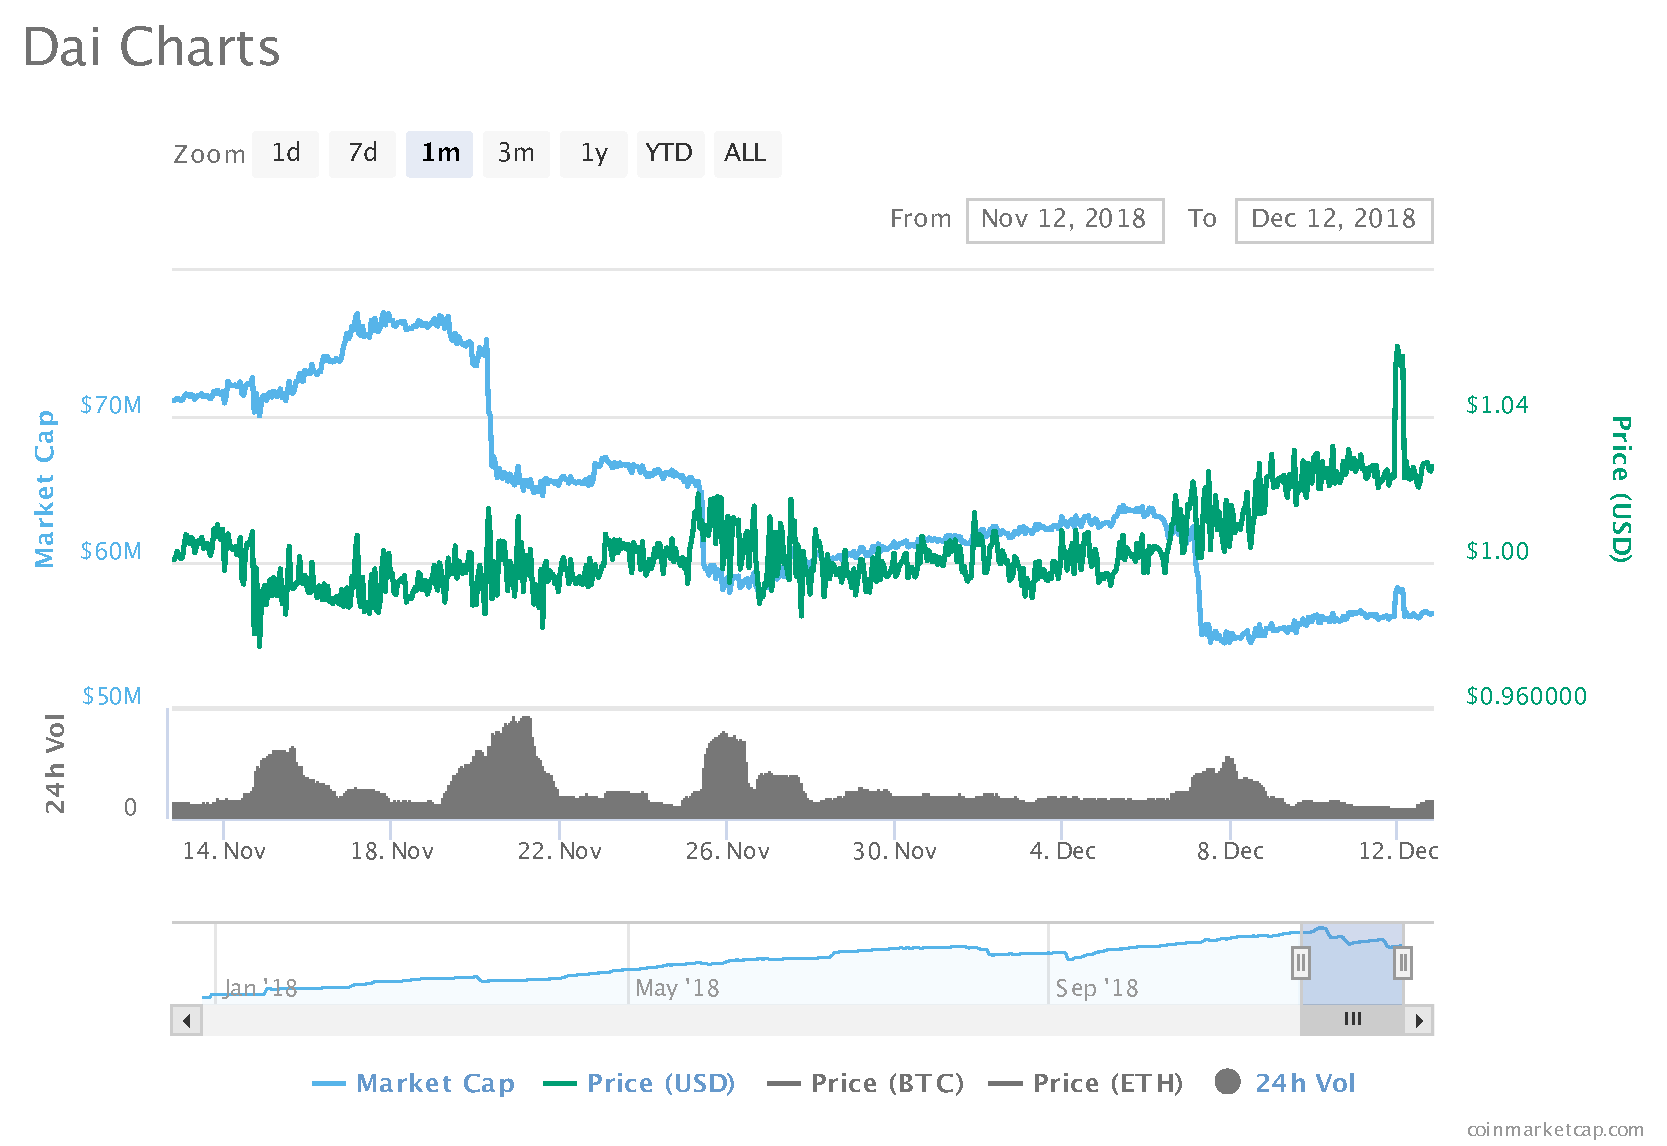
\includegraphics[width=9cm]{dai_chart}
	\caption{Dai price appreciates as speculators decrease supply--a potential feedback loop.}\label{fig:dai_chart}
\end{figure}


The stablecoin holder in this model essentially gives up all potential returns in exchange for `medium' volatility insurance. However, in large volatility events, the stablecoin takes on the direct tail risk of cryptocurrencies. As a result, the expected return of the stablecoin should in fact be negative as it is either worth the target price--e.g., \$1-- or, in the tail, significantly less.


Examples include \href{https://makerdao.com/dai}{MakerDAO's Dai} and \href{https://bitshares.org/technology/price-stable-cryptocurrencies}{bitUSD}. \href{https://www.steem.center/index.php?title=Steem_Dollar_(SBD)}{Steem Dollars} follows a similar but slightly different model. All Steem holders essentially back Steem Dollars, which are payed as rewards on the Steem platform. Steem dollars can be redeemed for \$1 worth of newly minted Steem, and so redemptions affect all Steem holders via inflation. BitUSD and Steem Dollars have broken their USD pegs as of Dec. 2018.


\subsection{Decentralized central bank}
In the decentralized central bank model, some DAO or smart contract algorithm attempts to control the coin supply--increasing or decreasing the coin supply as demand changes--with the aim that the market price of the stablecoin remains close to a target. In a manner similar to fiat currency, trust in the system is required in the initial setup of the stablecoin to assert the prescribed value. Following the initial setup, the system attempts to dynamically increase/decrease the coin supply in response to demand in the following ways:
\begin{compactitem}
	\item Should the price increase above the target, the system creates new coins to increase the coin supply until the price regains an equilibrium around the target. These new coins are awarded to stakeholders in the system, such as the owners of some sort of investment token or miners.
	\item Should the price decrease below the target, the system attempts to reduce supply in some of the following ways:
	\begin{compactitem}
		\item The system attempts to sell bond tokens that incentivize stablecoin holders to destroy their stablecoins in exchange for future interest, thereby decreasing the money supply. This bond interest is paid the next time the system mints new stablecoins to increase the coin supply (importantly, this is not guaranteed to happen).
		\item In some implementations, some proceeds from prior coin sales may be used to buy back stablecoins directly to reduce supply. In this case, the system can be thought of as under-collateralized with cryptoassets.
		\item In other implementations, a transaction fee is imposed to burn coins to reduce the coin supply.
	\end{compactitem}
\end{compactitem}
To operate in a decentralized manner, either a DAO determines when actions are taken or smart contract logic makes these decisions algorithmically.

\paragraph{Risk of catastrophic failure} I see the following problems with this:
\begin{compactenum}
	\item The bonds are in fact very risky derivatives. If the market for these dries up, as is prone to happen during extreme events, the stablecoin collapses. Thus any growth is likely transient. The alternative transaction fee to burn coins doesn't get around this problem. On one hand, it may not be enough supply reduction to counteract an extreme movement. On the other hand, it only places extra stress on the stablecoin market, which could dry up and exacerbate the problem.
	\item Any profit from transient growth in the system is purely extracted by investors when they receive and sell new stablecoins. Stablecoin holders have no claim to the value of this growth as there is nothing collateralizing the coins.
	\item The stablecoin relies on trusted oracles to provide real world price data, as in the decentralized collateral model. Oracle manimuplation could directly trigger a market failure event.
\end{compactenum}


The stability of these systems works perfectly if prices get too high--just mint new coins and give profits to stakeholders. However, in the downward direction, stability relies on having enough agents willing to take the risks associated with the bond positions and even just holding stablecoins, which turn out to bear the tail risk in the system. The bonds' future interest relies on the system recovering--i.e., the price rising above target again so that the system mints new coins to award bond holders. Agents may not be willing to bet on these bonds during extreme events that affect faith in the system or cryptocurrencies in general. This self-fulfilling issue shouldn't come as a surprise as the same issues affect central banks' control of fiat currencies (although of course in that case, the currencies also have the backing of powerful governments and transient profits aren't extracted by investors).

In essence, these stablecoins, which prescribe value out of thin air and are sort of `self-collateralized', are very similar to the decentralized collateral stablecoins, which are based on blockchain networks that have already done the value creation.\footnote{Note that this point isn't criticism: everything must start at this point somewhere.} Stakeholders in both systems receive income when new coins are sold and face a loss of their input should the system fail. And again the stablecoin holder gives away all potential return in exchange for `medium' volatility insurance while retaining the tail risk of something like cryptocurrencies.

Examples of these projects include \href{https://nubits.com/}{NuBits}, \href{https://www.basis.io/}{Basis}, and \href{https://www.kowala.tech/}{Kowala}. I address these in more detail in the Medium article \href{https://medium.com/@aklamun/basis-basecoin-is-a-bob-rubin-trade-8c5b8af2a18b}{``Basis/Basecoin is a Bob Rubin Trade''}. As mentioned above, NuBits has already failed and Basis recently decided to close down and return money to investors.








\subsection{CDO of stablecoins}
A \href{https://ethresear.ch/t/collateralized-debt-obligations-for-issuer-backed-tokens/525}{proposal by Vitalik Buterin} involves creating a collateralized debt obligation (CDO) structure around a portfolio of stablecoins that are not likely to fail together. This would be stronger than any individual underlying stablecoin. This would work in the following way:
\begin{compactenum}
	\item Say there are $n$ stablecoins. We create a CDO structure in which there are $n$ seniority tranches.
	\item At the end of the CDO term, the most senior tranche can select one of the $n$ stablecoins in the portfolio and receive it as payout. Thus the senior tranche only loses value if all $n$ stablecoins fail.
	\item In order of seniority, the next tranches choose one remaining stablecoin as payout.
\end{compactenum}
As the portfolio losses must be borne by someone, the senior tranches would pay some compensating interest to the lower tranches. Stablecoin holders would choose the tranche that suits their risk profile.

\paragraph{Issues}
This CDO approach presents some issues that make it less desirable:
\begin{compactitem}
	\item Holders of the safe assets (the most senior tranches) essentially face a negative interest rate. The security of these tranches would require significant compensating payments to the lower tranches. This may be ok as a last resort but goes against the spirit of a good store of value.
	
	\item The CDO system relies on enough agents being willing to bear the risks from the lower tranches. As before, during extreme events, these markets might dry up, in which case the CDO structure can't be renewed and senior tranche holders face the tail risk of cryptocurrencies upon expiration.
	
	\item For the reason above, it would be difficult to implement an indefinite-term stablecoin that is renewed in an algorithmic manner.
\end{compactitem}


%%%%%%%%%%%%%%%%%%%%%%%%%%%%%%%%%%%%%%%%%%%%
\section{New Design Proposal}\label{sec:new_design}

I propose a new stablecoin design that addresses the failure points of current designs by
\begin{compactenum}
\item Decoupling the ability to maintain a stability target from the ability to maintain market liquidity (and so incentives are always aligned to maintain the market)
\item Diversifying tail risks to the extent possible
\item Using blockchain to solve a tragedy of the commons problem (as defined below), retaining the profits of the system to fund a systemic insurance that is anti-fragile (i.e., grows in value during extreme events)
\item Avoiding/mitigating oracle manipulation risk by developing on-chain stability measures.
\end{compactenum}
This design works on two different levels. 

\paragraph{Meta-token structure}
On the first level, we spread risk between a number of cryptocurrency systems and/or tokenized real world assets with a token portfolio that serves as collateral for our new stablecoin (this is really an `easy pickings' improvement). These tokens have different tail risks (e.g., volatile crypto risk vs. counterparty risk), so there are gains from diversification (item 2). The end result can be free of specific counterparty risk to an acceptable degree if the diversification accounts for shared organization and jurisdictional relationships between centralized coins.

This collateral token portfolio is structured in an ETF-like way. That is, shares of the portfolio are separate tradeable meta-tokens that have a fundamental value tied to the value of the portfolio. The price of the meta-asset can diverge from the prices of the portfolio assets depending on market conditions. When this happens, a true arbitrage opportunity (i.e., a gain from a risk-free trade) is available. If the meta-token price is above fundamental value, an additional meta-token could be created and sold for more than the cost of underlying collateral. If the meta-token price is below fundamental value, a meta-token could be purchased and its collateral redeemed and sold for a profit. The `everyday target' of the new stablecoin is maintained by the incentives of this true arbitrage to keep the trading price in line with the fundamental value of underlying tokens (first part of item 1).

\paragraph{Rainy day fund}
On the second level, the stablecoin system is designed so that these arbitrage profits are partly retained by the system as a `rainy day fund'. This rainy day fund is used to maintain the long-term stability target (second part of item 1). The value of this arbitrage is anti-cyclic because the largest price deviations are expected to occur during and after extreme events--i.e., when there are rushes into and out of stable assets. The rainy day fund will tend to increase in value over time and especially during crises. Should collateral tokens fail, the rainy day fund is used to recapitalize the collateral portfolio to maintain the stability target.

In a normal financial system, this idea of systemic insurance is subject to the tragedy of the commons--it can benefit everyone communally but, individually, everyone has an incentive to skirt the rules to avoid paying. Blockchain provides a unique setting to solve this problem by making communally good rules ungameable (item 3). The rules of meta-token creation and redemption can be set such that arbitrage profits have to be funneled to the rainy day fund. This process can even be automated as smart contract vending machines without relying on human traders.

\paragraph{On-chain stability measure}
The stability target (usually USD) of all existing decentralized stablecoins involves trusting an oracle to provide USD-price data to the blockchain. I propose to avoid (or at least mitigate) this risk by leveraging economic data that is entirely on-chain to create measures of stability that do not require oracles (item 4). For instance, Ethereum gas prices tell us (loosely, as market dynamics also play a role) about the cost of real world computing power in terms of ETH. The right average window of gas prices would be a difficult measure to game and could provide an ETH price of something relatively stable. The ETH trading price of other tokens is available on-chain via decentralized exchanges. Together, these allow a stability measure of the collateral portfolio, which can be used for invoking the rainy day fund.

In the intermediate term, this might not be the best measure of stability because changes in gas prices don't completely reflect changes in ETH value. However, it can still be used as a rough check against oracle manipulation. In the long-term, when an established cryptoeconomy exists, even more economic information will be available on-chain, which might realistically provide the best stability measures. I believe a long-term evolution of a stablecoin like this one will eventually allow a new and transparent form of monetary policy by targeting agreed-upon measures of on-chain economic activity.





%%%%%%%%%%%%%%%%%%%%%%%%%%%%%%%%%%%%%%%%%%%%
\section{Proposed Research}\label{sec:proposed_research}

\paragraph{Research vision}
This project will perform foundational research on understanding how stablecoin markets work. There will be a substantial market design component to this research. Market design is a new field at the intersection of economics and computer science that studies why some markets work well and others do not, and how broken markets can be fixed. As systems can be quite large and complex, market design has a substantial computer science side, involving graph theory, complexity, and algorithms. In stablecoin markets, these systems are composed of complex algorithmic derivatives. This research will involve modeling stablecoin markets to compare different design characteristics. The aim is to understand the failure points of existing designs more formally, validate the design I propose (or improve on it), and tune the design parameters to work well in real markets.

\paragraph{This grant}
As a step in this direction, I propose an agent-based model that explores the complex interactions of various agents in a stablecoin market. The development and analysis of this model will be the focus of this grant. This work will build off of agent-based modeling in traditional financial markets--e.g., \citep{farmer15}.

The model will involve a number of agents with differing risk profiles, including those who desire to hold stablecoins and those who desire to speculate on the market, and heuristics for how these agents make decisions and learn from the past history. As these models simplify decision-making, it is key that their construction is well motivated. Design and parameter choices need to be defensible for deriving insight into real world settings. This will be a primary focus of the model development. I will use Lykke data (such as public tradelog data), among other datasets, to calibrate the model.

Agent-based models allow tractable simulation of complex interactions and, in some simple cases, analytical study of the resulting dynamical systems. They can be used to test how changes in individual behaviors and system design can affect the emergent behavior in a controlled environment. I will analyze the systems resulting from various designs, study their long term behaviors, learn about the conditions under which these systems function and fail, and learn which design characteristics tend to make stronger systems.

I argue that such a model can be a good simplified framework for initializing this area of research. Generally, tractable game-theoretic models that depend on human judgment and market confidence have proven difficult to develop in this area \citep{sok15}. These are part of significant open problems, which I intend to tackle in follow-up work.

Additionally, I aim to foster a community around rigorous stablecoin research. I am not aware of any significant research work in this area--only the existing development projects that I address in Section~\ref{sec:existing_designs}. As stablecoins become increasingly popular, I think this is a critical missing piece in the ecosystem. I have already started this community in finding interested research collaborators and sharing my ideas. I will continue by sharing this work with a larger audience at conferences and workshops.


\paragraph{Milestones} This work will concentrate on the first half of the Spring 2019 semester with follow-up work continuing after.

\textbf{3 months -- First paper completed}. This milestone is the focus of this grant. The paper will focus on the agent-based model of stablecoin markets and understanding how various designs fail in crises. I will also write a corresponding blog post describing the major points in a more colloquial manner.

If the results suggest that a first prototype of a new design would be a valuable next step, I will develop this next. This will be released as an open source project that will be the basis for ongoing community collaboration so that anyone who is interested can begin participating. Alternatively, I will begin work on more advanced stablecoin market models.

\textbf{6 months -- Present first paper}. I aim to present the first paper at an upcoming National Bureau of Economic Research conference on blockchain and financial contracting and at an INFORMS (Institute for Operations Research and the Management Sciences) conference.

This work will be followed by the development of more advanced stablecoin market models, such as game-theoretic equilibrium models, and further study of stablecoin market design. My research focus is to develop and validate better stablecoin designs. When satisfactory progress has been made on that front, I will work to implement what we have learned. This would be a point at which the project could be sustained through outside investment.




\begin{thebibliography}{}
	
	\bibitem[Aymanns and Farmer, 2015]{farmer15}
	Aymanns, C., Farmer, D.J. (2015).
	\newblock The dynamics of the leverage cycle.
	\newblock {\em Journal of Economic Dynamics \& Control}, 50:155--179.
	
	\bibitem[Bonneau et~al., 2015]{sok15}
	Bonneau, J., Miller, A., Clark, J., Narayanan, A., Kroll, J., Felten, E. (2015).
	\newblock SoK: Research perspectives and challenges for Bitcoin and cryptocurrencies.
	\newblock {\em 2015 IEEE Symposium on Security and Privacy}.
	
\end{thebibliography}



\end{document}
